%----------------------------------------------------------------------------
\chapter{Irodalmi áttekintés}
%----------------------------------------------------------------------------

\section{Mobil robotok irányítása}
A mobil robotok irányítása alapvető szerepet játszik az autonóm rendszerek hatékony működésében. Az autonóm mobil robotok  alkalmazási területeik két részre bonthatók, az egyik az olyan feladatok, amelyek nagy precizitást igényelnek és egy embernél gyorsabban, pontosabban szükségesek elvégezni, a másik a könnyen autómatizálható feladatok, ahol robotok alkalmazásával jelentős költségmegtakarítás érhető el. Például:

\begin{itemize}
    \item \textbf{Logisztika}: Raktári robotok optimalizálják az áruk szállítását, csökkentve az emberi erőforrás szükségletét és növelve a hatékonyságot.
    \item \textbf{Egészségügy}: Autonóm robotok biztosítják a steril környezetet és az időérzékeny anyagok szállítását kórházakban.
    \item \textbf{Mezőgazdaság}: Robotok segítenek a precíziós gazdálkodásban, például a növények állapotának monitorozásában vagy a gyomirtásban.
\end{itemize}

Az autonóm mobil robotok sikere nagyban függ a vezérlési rendszer minőségétől. Egy hatékony irányítórendszer:
\begin{enumerate}
    \item \textbf{Pontosan vezérli a robot mozgását} a megadott pályán.
    \item \textbf{Akadályokat kerül el biztonságosan}, az emberi és környezeti tényezőket figyelembe véve.
    \item \textbf{Döntéseket hoz valós időben} a változó környezetben.
    \item \textbf{Energiahatékony} működést biztosít, ami különösen fontos akkumulátorról működő rendszerek esetén.
\end{enumerate}

A mobil robotok irányítása különösen bonyolult, mivel figyelembe kell venni:
\begin{itemize}
    \item a robot kinematikai és dinamikai modelljét,
    \item a környezeti bizonytalanságokat, például dinamikus akadályokat,
    \item a rendszer korlátait, mint például a szenzorok pontosságát és a robot fizikáját.
\end{itemize}

\section{Robotok mechanikai felépítése}
Robotok mechanikai felépítésük alapján kétféle csoportra oszthatók: térbeli mozgásra képes és mozgásra nem képes alappal rendelkezők. A fix alaphoz kötött robotok geometriai felépítése leírható merev testek (links) és csuklók (joints) kapcsolatainak sorával, melyek egy adott munkatérben képesek mozogni. A mozgó alappal rendelkező robotok a térben helyet tudnak változtatni. Mechanikai szempontból egy vagy több merev testből állhatnak, melyekhez csatlakozik egy elmozdulásra képes rendszer például kerekek. \cite{siciliano2010robotics}

\subsection{Mobil alappal rendelkező robotok}
Mobil robotok tovább csoportosíthatók kerekekkel (vagy valamilyen elforduló mechanizmussal) vagy lábakkal mozgó osztályokra. Továbbiakban a kerekekkel rendelkező robotokról lesz szó, mivel ez az osztály lényeges a diplomamunka szemszögéből. Az ilyen robotok különféle kerék mechanizmusokkal szerelhetők fel, ahogyan a képen (\refstruc{fig:wheels}) is látható:
\begin{figure}[!ht]
    \centering
    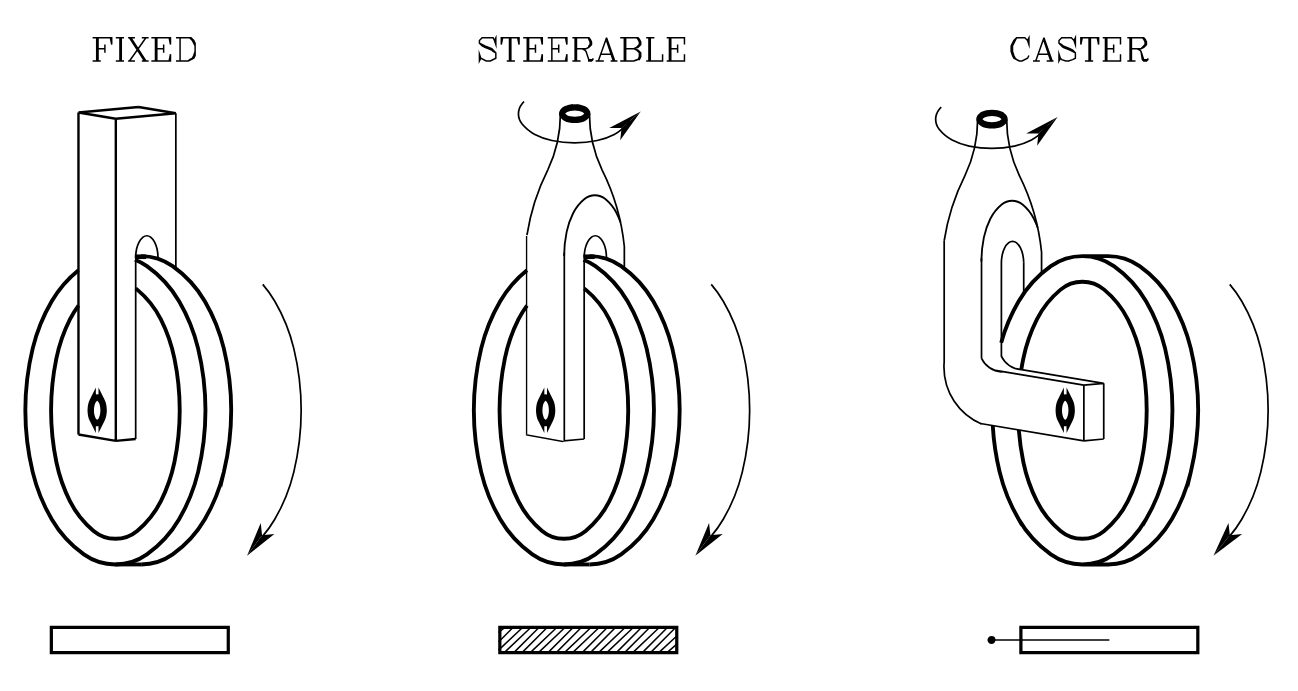
\includegraphics[width=150mm, keepaspectratio]{figures/021_wheels.png}
    \caption{Kerék mechanizmusok \cite{siciliano2010robotics}}
    \label{fig:wheels}
\end{figure}

\begin{itemize}
    \item \emph{Fix kerekek (fixed)}: csak irányban forognak (előre-hátra), nem képesek elfordulni oldalirányban. Általában meghajtott kerekek tartoznak ide, amelyek a robot hajtását biztosítják, például egy autó hátsó tengelyére szerelt kerekek. A robot bázisához mereven csatlakoznak és saját tengelyük körül forognak, amely ortogonális a kerék síkjára.\cite{siciliano2010robotics}
    \item \emph{Kormányozható (steerable) kerekek}: oldalirányban elfordíthatók, a haladási irányuk megváltoztatható, például autó első tengelyén lévő kerekek. A robot bázisához egy csuklóval csatlakoznak, mely lehetővé teszi a kerekek elfordulását, illetve erre merőleges saját tengellyel rendelkeznek (szintén merőleges a kerék síkjára), melyek körül forognak.\cite{siciliano2010robotics}
    \item \emph{Szabadonfutó (bolygó/caster) kerekek}: hasonló mechanikai csatlakozással rendelkeznek, mint az irányítható kerekek, azonban a robot bázisához való csatlakozásuknál található tengely körül szabadon fordulnak el, például irodai székek vagy bevásárló kocsi kerekei. A vertikális tengely nem metszi a kerék elfordulási tengelyét hanem egy "offset" távolságra helyezkedik el. Ezek a kerekek mechanikai stabilitásban segítik a robot bázist.\cite{siciliano2010robotics}
\end{itemize}

\subsection{Mobil kerekes robotok kinematikai modellje}
Kétféle csoportosítás különíthető el: holonomikus (nem tud mozogni a sík bármelyik irányában) és omnidirekcionális (tetszőleges irányba képes mozogni). Omnidirekcionális robotok mecanum (másik nevén svéd) kerekekkel (\refstruc{fig:023_omni_wheel}) felszerelt robotok, melyek több forgó alkatrésszel rendelkeznek, a kerék kerületen mentén független elfordulni képes görgők vannak amik segítségével oldalazó mozgást is végezhet a kerék tengelyével párhuzamosan. \cite{siciliano2010robotics} \cite{ros2_control_docs}

\begin{figure}[!ht]
    \centering
    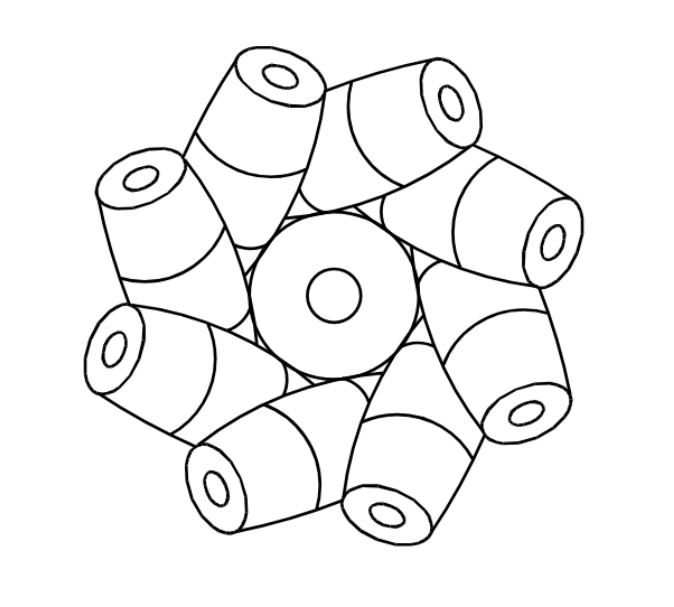
\includegraphics[width=75mm, keepaspectratio]{figures/023_omni_wheel.png}
    \caption{Mecanum kerék \cite{siciliano2010robotics}}
    \label{fig:023_omni_wheel}
\end{figure}

A dolgozatban vizsgált robotmodellek holonomikusak. Több fajta (előző pontban tárgyalt) kerék elrendezéssel hozható létre ilyen robotmodell. Klasszikusan a tricikli modell (\refstruc{fig:024_tricikli_car}), amely egy tengelyen két együttesen meghajtott kerékkel rendelkezik és egy kormányzott kerékkel. Az autókhoz hasonló modellek négy kerékkel (\refstruc{fig:024_tricikli_car}) ahol ebből kettő meghajtott és kettő kormányozható, vagy kettő egyszerre kormányozható és meghajtott plusz kettő stabilitásban asszisztáló fix kerékkel. Differenciál hajtású mobil robotok (\refstruc{fig:025_diff_model}) is a holonomikus robotok közé tartoznak, melyek két függetlenül meghajtott kerékkel és egy vagy több szabadon elforduló kerékkel szerelnek fel.  \cite{siciliano2010robotics} \cite{ros2_control_docs}

\begin{figure}[!ht]
    \centering
    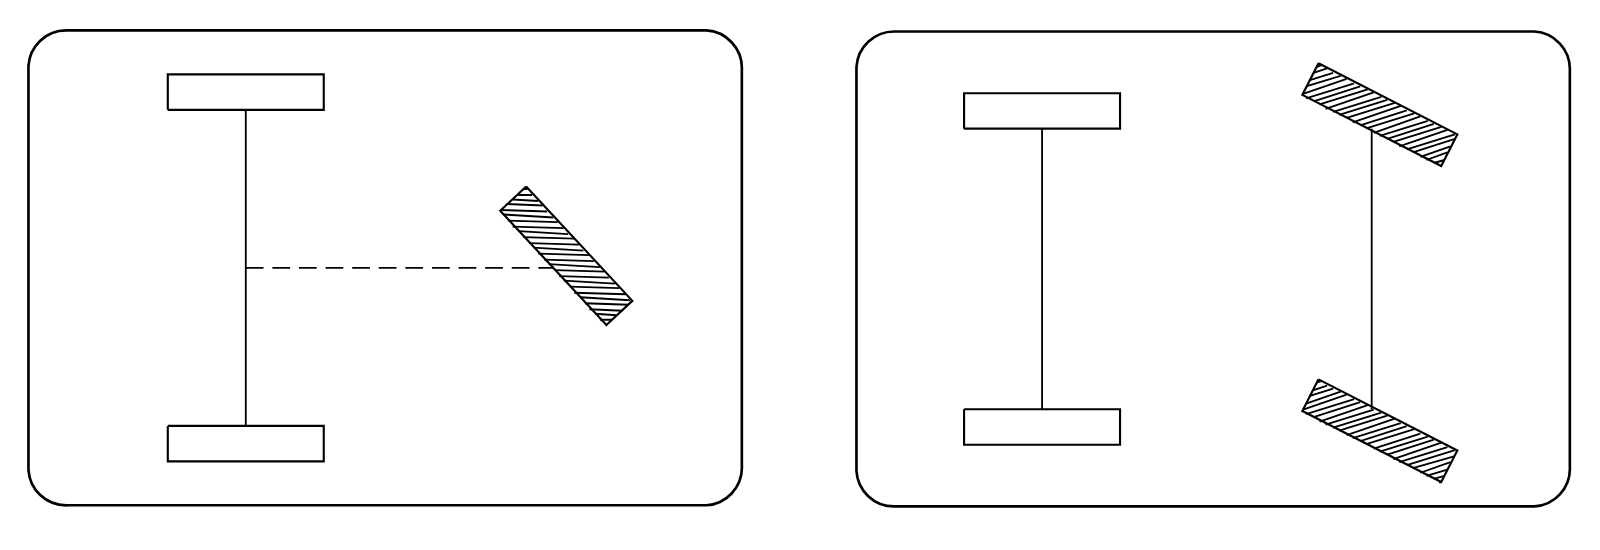
\includegraphics[width=150mm, keepaspectratio]{figures/024_tricikli_car.png}
    \caption{Tricikli és autó modellek \cite{siciliano2010robotics}}
    \label{fig:024_tricikli_car}
\end{figure}

\subsection{Differenciál hajtású robotok}
TODO: források
% Siegwart, R., Nourbakhsh, I. R., & Scaramuzza, D. (2011). Introduction to Autonomous Mobile Robots. MIT Press.
% Bekey, G. A. (2005). Autonomous Robots: From Biological Inspiration to Implementation and Control. MIT Press.

A diplomamunka során használt robotok közül mindegyik ebbe a kategóriába esik. Két szeparáltan meghajtott kerekének köszönhetően egyhelyben képesek megfordulni. A forgás tengelye a két kerék tengelyének közzéppontja. A passzív caster kerék vagy kerekek a stabilitásban segítenek, ezek lekövetik a robot mozgását. Ugye egy sík három pontból már felírható ezért a robot statikai egyensúlya nem jelent problémát, amíg a tömegközéppont vetülete a mozgás síkjára a három vagy több kerek talajjal való találkozási pontjainak egyenes szakaszokkal összekötő polinom belsejében marad. Mint mobil robot a differenciál hajtású szerkezetek munkatere virtuálisan végtelen, ha a munkateret a környezet egy altereként értelmezzük. A valóságban természetesen előjönnek olyan korlátok, mint a robot fizikai kiterjedése és a környezetben lévő akadályok relatív mérete és pozíciója. Természetesen itt sík felületet feltételezve (és kizárva lépcsőket, lifteket stb.) Mint nem omnidirekcionális robotmodell a lokális elmozdulására esnek korlátok. Nem tud rögtön a hajtott kerekek tengelyére merőleges irányába elmozdulni, ehhez szükséges fordulnia. De képesnek tekinthető bármely pozíciót felvenni csak nem rögtön. Ez úgy is kifejezhető, hogy a robot szabadsági fokainak száma alacsonyabb, mint a pozíciót leíró vektor változói. \cite{siciliano2010robotics} \cite{ros2_control_docs}

\begin{figure}[!ht]
    \centering
    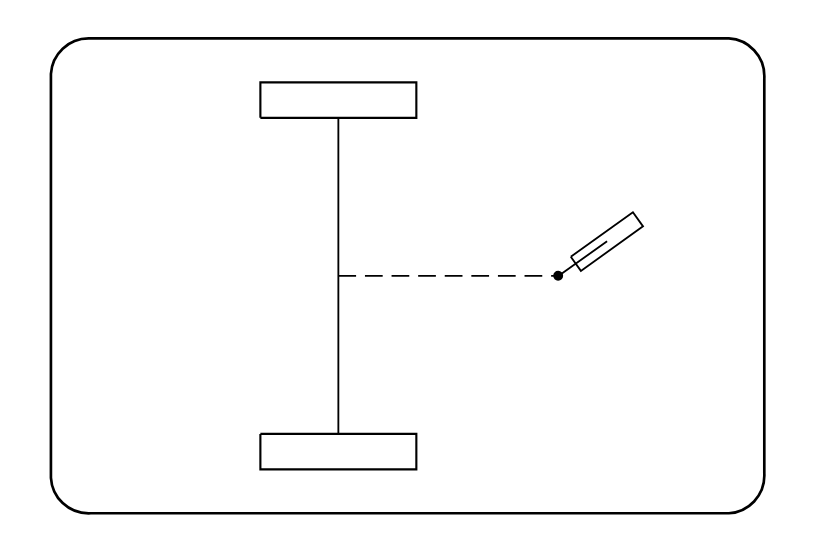
\includegraphics[width=75mm, keepaspectratio]{figures/025_diff_model.png}
    \caption{Differenciál hajtású robot modell \cite{siciliano2010robotics}}
    \label{fig:025_diff_model}
\end{figure}

A differenciál hajtású robotok számos előnnyel rendelkeznek más mechanikai felépítésekkel szemben, amelyek közül az egyik legkiemelkedőbb a szerkezet egyszerűsége. A két különálló hajtott kerék és a passzív támasztó kerekek kombinációja mechanikailag egyszerű és költséghatékony megoldást kínál, amely csökkenti mind a gyártási, mind a karbantartási költségeket. Ez a kialakítás különösen előnyös az oktatási és kutatási célú alkalmazásokban, ahol a költséghatékonyság kiemelt szempont.

Ezen kívül a differenciál hajtású robotok manőverezési képességei kimagaslóak. A két hajtott kerék lehetővé teszi, hogy a robot helyben forduljon, azaz nulla sugarú fordulást hajtson végre, ami rendkívül hasznos szűk helyeken történő navigáció során. Ez a képesség különösen beltéri környezetben, például raktárakban, laboratóriumokban vagy otthoni robotikai alkalmazásokban biztosít jelentős előnyt.

Energiafelhasználásuk szintén kedvező. A differenciál hajtású rendszerek egyszerű hajtásmechanizmusa kevésbé energiaigényes, mint a komplexebb robotmechanizmusok, például a lánctalpas vagy az omnidirekcionális rendszerek. Emellett stabilitásuk is kiemelkedő: a három vagy több támasztópont miatt a robot mozgása stabil, feltéve, hogy a súlypontja a támasztópontok által határolt területen belül helyezkedik el.

Ugyanakkor vannak hátrányai is ezeknek a rendszereknek, különösen más, fejlettebb mechanizmusokkal összehasonlítva. A differenciál hajtású robotok nem omnidirekcionálisak, azaz nem képesek azonnal bármely irányba mozogni. Mozgásuk gyakran több lépést igényel, mivel a hajtott kerekek tengelyére merőleges irányú elmozduláshoz először el kell fordulniuk. Ez korlátozza mobilitásukat dinamikus és változó környezetekben, ahol gyors irányváltásokra van szükség. Ez kihívást nyújt különböző szabályzók tervezésekor, használatakor.

Ezenkívül a differenciál hajtású robotok mozgása sík terephez kötött, ami akadályokkal vagy egyenetlen talajjal tarkított környezetben problémát jelenthet. Fizikai korlátok akadályozhatják nehezebb tárgyak szállításában, szemben például a lánctalpas robotokkal. Továbbá, csúszós felületeken, például koszos vagy nedves padlón, fordulás közben a kerekek megcsúszhatnak, ami pontatlan manőverezést eredményezhet. Ezek olyan problémák, amik kezelhetőek, de fontos megjegyezni, hogy el nem hanyagolhatók. Például nehezebb terhek szállításánál a kerekek terhelése nőhet, ezért opcióként kell tekinteni több bolgyó kerék beépítésére. A talaj és hajtott kerekek közötti súrlódás növelése érdekében a kerekek anyagát és mintázatát is figyelembe kell venni, illetve nem hanyagolható el a gondolat és igény a szoftveres kerék kicsúszás detektálásra és abból eredő korrigálásra, aminek szintén megvannak a maga eszközei, korlátai.

Összességében a differenciál hajtású robotok egyszerűségük, hatékonyságuk és könnyű kezelhetőségük miatt kiváló választást jelentenek számos alkalmazási területen, azonban érdemes figyelembe venni a mobilitásukból és környezeti korlátaikból adódó hátrányokat is. Egy tipikus példa a TurtleBot\footnote{TurtleBot: \url{https://www.turtlebot.com/}}sorozat, amelynek egyszerű és hatékony kialakítása ideális oktatási célokra és beltéri autonóm navigációra. Diplomamunka során három differenciál hajtású robotmodellt használtam. Ebből kettő TurtleBot hármas szérájából a waffle és burger model és egy méretében nagyobb robotmodellt, melynek fejlesztésén munkahelyemen dolgozok. Ezekre később részletesen kitérek, viszont itt szeretnék egy rövid ismertetést írni a TurtleBot-okról.

TODO: képek (tb3 burger waffle)

A TurtleBot egy alacsony költségű, személyes robotkit, amely nyílt forráskódú szoftverrel érkezik, és kifejezetten oktatási, kutatási, hobbi és prototípusfejlesztési célokra tervezték. A diplomamunkám során a TurtleBot 3-as verzióját használtam, azon belül is a Burger és Waffle modelleket. A TurtleBot 3 célja, hogy jelentősen csökkentse a robotplatform méretét és árát, miközben megőrzi a funkcionalitást és minőséget, valamint lehetőséget biztosítson a bővíthetőségre. A robot platformja rugalmasan alakítható át a mechanikai részek újraszerkesztésével (akár otthoni 3D nyomtatott alkatrészekkel) és különböző szenzorok, mikrovezérlővel vagy elektronika hozzáadásával.

TODO: forrás: TurtleBot Inventors Tell Us Everything About the Robot (IEEE Spectrum, By Evan Ackerman, 26 Mar 2013)
https://spectrum.ieee.org/interview-turtlebot-inventors-tell-us-everything-about-the-robot

\subsection{Differenciál hajtású robotok mozgásegyenletei}
TODO: források
% Roland Siegwart, Illah R. Nourbakhsh, Davide Scaramuzza
% Introduction to Autonomous Mobile Robots
% MIT Press, 2011.
% Autonomous Robots: From Biological Inspiration to Implementation and Control
% MIT Press, 2005.

A differenciál hajtású robotok mozgását a kinematikai modelljük írja le, amely az egyes kerekek sebességének és a robot általános mozgási paramétereinek kapcsolatát adja meg. Ezeket a mozgásegyenleteket arra használjuk, hogy a robot mozgását leírjuk, vagy vezérlési parancsokat generáljunk a kívánt mozgás eléréséhez. A mozgásegyenletek alapja, hogy a robot egy síkon mozog, két hajtott kerékkel és esetleg további szabadonfutó kerekekkel van felszerelve.

\begin{figure}[!ht]
    \centering
    \includesvg[scale=1.2]{figures/022_diff_drive.svg}
    \caption{Differenciál hajtású robot 2 dimenzióban \cite{ros2_control_docs}}
    \label{fig:022_diff_drive}
\end{figure}

A \refstruc{fig:022_diff_drive} jelölései a következők. A $v_{right}$ és $v_{left}$ a jobb, illetve bal oldali kerék kerületi lineáris sebessége. Ez a sebesség a kerék érintkezési pontján mért, a kerék síkjára merőleges érintőirányú sebesség, amely meghatározza, hogy a kerék milyen gyorsan halad előre (vagy hátra) a talajon. Az SI mértékegységük $\mathrm{m/s}$. A kerületi sebességek ($v_{right}$ és $v_{left}$) közvetlenül kapcsolódnak a kerék forgási sebességéhez, valamint a kerék sugarához az összefüggés $v = \omega r$ alapján, ahol $\omega$ a forgási sebesség (kerekeké), $r$ pedig a kerék sugara. $v_x$: a robot bázispontjának lineáris sebessége a robot $x$ tengelye mentén. Ez a robot középpontjára vonatkozó előrehaladási sebesség, amely a két kerék sebességének átlaga alapján számítható ki. Az SI mértékegysége $\mathrm{m/s}$.
$\omega_z$: a robot szögsebessége a $z$ tengely körül (amely a síkból felfele mutat). Ez a robot forgási sebessége, amely a két kerék közötti sebességkülönbségen alapul. Az SI mértékegysége $\mathrm{rad/s}$. $w$: a két hajtott kerék tengelyei közötti távolság (nyomtáv). Ez egy statikus paraméter, amely a robot mechanikai kialakításától függ. Az SI mértékegysége $\mathrm{m}$. Ezek a változók szolgálnak a robot aktuális mozgásának modellezésére. S az alábbi mozgásegyenletekkel írják le a robot mozgását:
\begin{align}
    v_{x}      & = \frac{v_{right} + v_{left}}{2}, \\
    \omega_{z} & = \frac{v_{right} - v_{left}}{w}, \\
    v_{left}   & = v_{x} - \omega_{z} \frac{w}{2}, \\
    v_{right}  & = v_{x} + \omega_{z} \frac{w}{2}.
\end{align}

Az egyenletek értelmezése alapján $v_{left}$ és $v_{right}$ a bal és jobb oldali hajtott kerekek sebessége, amelyek a robot általános mozgásának eléréséhez szükségesek. Az egyenletek tehát lehetővé teszik a robot aktuális mozgásának leírását, valamint a kívánt mozgási paraméterek alapján a keréksebességek kiszámítását. Ezek az összefüggések elengedhetetlenek a robot vezérléséhez és navigációjához, valamint az autonóm mozgás tervezéséhez. A diplomamunka során használt robotok irányítása az $v_x$ és $\omega_z$ paraméterek segítségével oldaható meg. A szablyzónak ezeket az értékeket szükséges meghatározni, a mozgásegyenletek segítségével pedig a motorvezérlő vagy szimulációban differenciál hajtást biztosító pluigin feladatkörébe tartozik az egyes kerekek megfelelő sebességének ($v_{right}$ és $v_{left}$) beállítása.

\section{Robotok szabályozása}
A szabályozás kulcsfontosságú a mobil robotok működésében, mivel biztosítja a robot mozgásának stabilitását és pontosságát. Egy autonóm robotnak képesnek kell lennie arra, hogy különböző környezeti feltételek között is megbízhatóan navigáljon, miközben leköveti a kívánt pályát. A szabályozás feladata, hogy a robot kerekének sebességét és irányát dinamikusan módosítsa a kívánt mozgás eléréséhez. Az optimális szabályozás nélkül a robot mozgása instabillá válhat, például csúszás vagy pontatlan kanyarodás léphet fel. Egy jól működő szabályozási rendszer képes kompenzálni a szenzorokból és aktuátorokból származó hibákat, például a kerékcsúszást vagy a zajos pozícióadatokat. A differenciál hajtású robotok esetében a szabályozás különösen fontos, mivel a két hajtott kerék sebességének összehangolása határozza meg a haladási és forgási mozgásokat. A szabályozás lehetővé teszi a robot számára, hogy gyorsan reagáljon a környezet változásaira, például mozgó akadályok elkerülésére. Emellett a szabályozás biztosítja a robot energiahatékonyságát, optimalizálva a hajtáshoz szükséges erőforrásokat. A komplexabb környezetekben, például dinamikus akadályok vagy szűk helyek esetén, a szabályozási algoritmusok teszik lehetővé a robot biztonságos és precíz működését.

Különféle feladatkörök és igények különíthetők el egy autonóm navigáló robot esetében, melyek szétosztása nem a legtriviálisabb feladat, ilyenek lehetnek például a következők:
\begin{itemize}
    \item \textbf{Pályatervezés:} Két pont közötti legrövidebb és legbiztonságosabb (akadályok elkerülése szempontjából) útvonal meghatározása.
    \item \textbf{Pálya követés:} A robotnak a meghatározott pályán való haladásának biztosítása.
    \item \textbf{Kinematikai és dinamikai korlátok betartása:} A robot mozgásának sebesség vagy gyorsulás korlátok között tartása.
    \item \textbf{Akadályok elkerülése:} Dinamikus és statikus akadályok felismerése és kikerülése a mozgás során.
    \item \textbf{Valós idejű döntéshozatal:} A változó környezetben gyors és helyes döntések meghozatala a navigáció során.
    \item \textbf{Hibaelhárítás:} Hibás szenzoradatok vagy váratlan környezeti hatások kezelése, hogy a robot továbbra is folytathassa a feladatát.
\end{itemize}

Ezen feladatkörök többféle alrendszerben különülhetnek el. Tervezési kérdés, hogy melyikért mi felel.
A pályatervezés legtöbbször egy globális tervező feladata, amely az egész mozgástartományról készített reprezentációval dolgozik.

\section{Model prediktív szabályozás}
\section{MPPI}
- különbséges, hasonlóságok
- képeletek
\section{}